\chapter{Identifikáció}\label{chap:ident}


A szabályzó tervezésénél használt szakaszmodell a Simulinkben megvalósított fizikai modell viselkedését leíró lineáris rendszer. Ebben a fejezetben a korábbiakban ismertetett hálózatot identifikálom.

\begin{figure}[h]
	\centering
	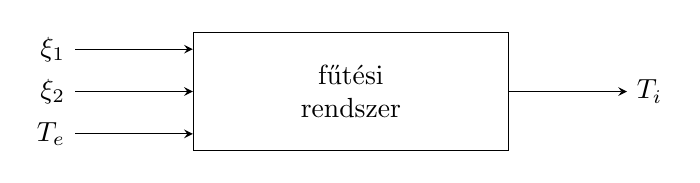
\begin{tikzpicture}[>=stealth,
	outer/.style={draw=gray,dashed,thick,inner sep=5pt}]
	
	% nagy blokkok
	\node[draw,rectangle, minimum height=1.5cm,minimum width=4cm] (plant) at (0,2.5) {\parbox{2cm}{\centering fűtési rendszer}};
	%\node[draw,rectangle, minimum height=1.5cm,minimum width=3cm] (Control) at (0,2.5) {\parbox{2.5cm}{\centering modellalapú\\szabályzó}};
	
	% szaggatott vonal
	%\node[draw,outer,rectangle, minimum height=4cm,minimum width=12cm,
	%label={[label distance=-0.1cm, anchor=north]100:Matlab Simulink szimuláció}] (keret) at (2.5,2.5) {};
	
	
	% plant bemenetei
	\draw [<-] (plant.165) node[left]{} -- +(-15mm,0) node[left]{${\xi_{1}}$};
	\draw [<-] (plant.180) node[left]{} -- +(-15mm,0) node[left]{${\xi_{2}}$};
	\draw [<-] (plant.195) node[left]{} -- +(-15mm,0) node[left]{$T_{e}$};
	\draw [->] (plant.0) node[left]{} -- +(15mm,0) node[right]{$T_{i}$};
	
	% szabályzó bemenetei
	% a -| és |- máshogy fog törni, ha unconstraintelt.
	%\draw [->] (plant.0)  node[left]{$t_i$} -|++(0.8,-1.5) -| ++(-9.25,0) |-  ++(-1.1,0) |- node[left]{$t_i$} (Control.198);
	
	%\draw [<-] (Control.180) node[right]{} -- +(-10mm,0) node[left]{$t_{e}$};
	%\draw [<-] (Control.162) node[right]{} -- +(-10mm,0) node[left]{$t_{ref}$};
	\end{tikzpicture}
	\caption{A szabályzott szakasz összevont modellje}
	\label{tikz:simulation}
\end{figure}


A Simulinkben vizsgálójeleket használok: a több bemenetű, egy kimenetű rendszert egyszerre csak egy bemenetén gerjesztem. A tömegáramot szabályzó szelepek nyitott és csukott állapot között folytonosan állíthatók, 0 és 1 közötti beavatkozó jellel. A külső hőmérsékletet a modell kelvinben kapja, kimenete a belső hőmérséklet. 

 %(\textit{\ref{fig:valve-step}. ábra}). 
% a kimeneti változást létrehozó hatás egyértelműen beazonosítható kell hogy legyen.

\section{A szakasz ugrásválasza}

Lineáris hálózatoknál gyakori vizsgálójel az egységugrás, illetve az impulzusgerjesztés. Az identifikációhoz ugrásválaszt vizsgáltam, de mivel a rendszernek 3 bemenete 

\begin{figure}[H]
	\centering
	% trim={<left> <lower> <right> <upper>}
	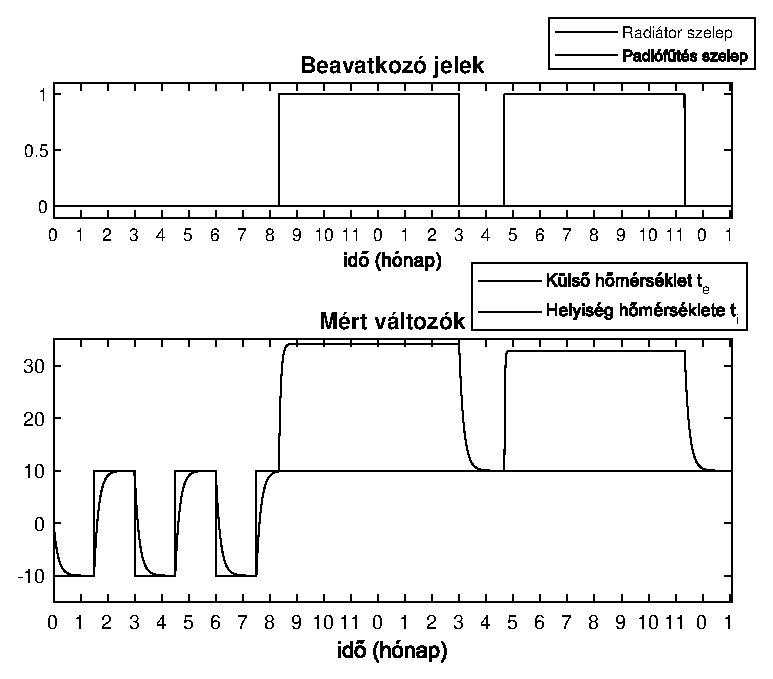
\includegraphics[trim=0 0 0 0, clip,width=0.9\textwidth]{figures/valve-step}
	\caption{Szimulációs eredmények a bemeneteket külön-külön gerjesztve}
	\label{fig:valve-step}
\end{figure}

A módszer az, amit a több forrást tartalmazó hálózatok esetén is alkalmazunk: a válasz számításakor mindig egy forrás hatását vizsgáltuk,  hálózatnak egyszerre csak egy bemenetét gerjesztem. Lineáris hálózat vizsgálatakor a kimeneten a válasz szuperpozícióval adódik. 

\begin{figure}[H]
	\centering
	% trim={<left> <lower> <right> <upper>}
	\includegraphics[trim=0 0 0 0, clip,width=0.9\textwidth]{figures/valve-stair}
	\caption{Szimulációs eredmények a szelepeket lépcsős függvénnyel gerjesztve}
	\label{fig:valve-stair}
\end{figure}

A fűtőtestekben a víz tömegáramát szelepekkel szabályozzuk. Az \textit{\ref{eq_holeadas4}. egyenlet} adja fűtőtestek által leadott hőmennyiséget, ám ez nem lineáris függvénye a tömegáramnak. A \textit{\ref{fig:valve-stair}. ábrán} látszik, hogy kétszer jobban kinyitott szeleppel $t_i$ belső hőmérséklet végértéke csak kicsivel lesz magasabb. Itt nem működik tehát a szuperpozíció elve, a bemenet a [0..1] tartományban sem lineáris\footnote{A szakasz másik nemlinearitása a szaturáció: a szelepet csak [0..1] tartományban lehet működtetni -- a szabályzótervezésnél ezt figyelembe fogom venni.}.

A $t_i$ belső hőmérséklet végértéke a tömegáramon kívül a $t_e$ külső hőmérséklettől is függ: ugyanakkora belső hőmérsékletet csak nagyobb tömegárammal, vagy nagyobb $t_w$ előremenő vízhőmérséklettel lehet tartani\footnote{Bár a vízhőmérsékletet nem szabályozom, egyes kazánok rendelkeznek külső hőmérővel, így a vízhőmérsékletet megemelve a hidegben a $t_i$ végértéke "automatikusan" azonos maradhat.}. 

\begin{figure}[H]
	\centering
	% trim={<left> <lower> <right> <upper>}
	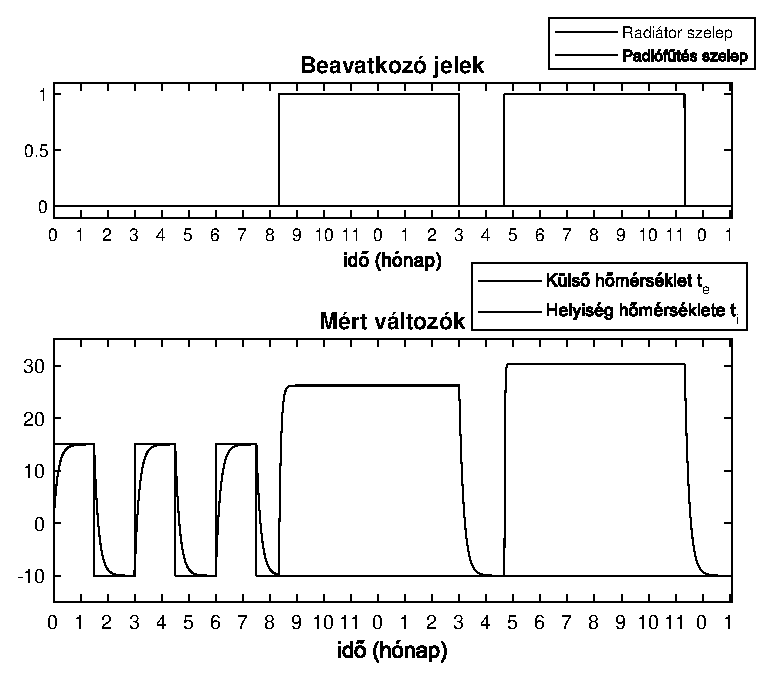
\includegraphics[trim=0 0 0 0, clip,width=0.9\textwidth]{figures/valve-step-hot}
	\caption{Szimulációs eredmények a bemeneteket külön-külön gerjesztve}
	\label{fig:valve-step-hot}
\end{figure}

Látható, hogy a különböző bemenetekre adott gerjesztések hatása a kimeneten nem számítható szuperpozícióval: \SI{20}{\celsius}-kal megemelt $t_e$ külső hőmérséklet esetén a fűtőtestek nem fognak \SI{20}{\celsius}-kal magasabb belső hőmérsékletre fűteni.

%A Simulink modellt bemenetein gerjesztem (külső hőmérséklet \SI{40}{\celsius}, majd fűtés \SI{60}{\celsius} előremenő hőmérsékleten valve = 1 állásban.\footnote{A stratégia lehet $t_s$ előremenő hőmérséklet vagy $\xi \cdot \dot m$ tömegáram szabályzása $\alpha$ = [0..1] beavatkozójellel. })


Az identifikációhoz adatfile-t hozok létre, a Simulinkben IDDATA blokk a be- és kimenetek értékét mintavételi időnként rögzíti és a \textit{Base Workspace}-be (a közös változók közé) menti. Innen a \textit{System Identification} app-ba betölthetők az adatok. %A mintavételi idő először egy másodperc volt. %A Matlab Workspace-ben megjelenik egy iddata, ezt tudom az ident toolboxba importálni.
Az adatsorra átviteli függvényeket illesztek: a pólusok, zérusok a száma a Simscape modell alapján meghatározható, RC-hálózatok analógiájával. Ekkor pl. a radiátorok felmelegedési idejét is leköveti a modell. A teljes helyiség időállandójához képest viszont pl. a radiátor felmelegedése elhanyagolható. Fél órás mintavételi idő esetén a fűtőtestek egytárolós taggal helyettesíthetők. 




Célszerű az identifikációnál minél nagyobb változásokat mérni - így a rendszer teljes dinamikáját, hőtároló képességét mértem. A beállási idők kb. 30 naposak voltak és több periódusnyi mérésre volt szükség. 


%Nem tartottam "értelmét" 1\si{\celsius}-os step jelre identifikálni. Így beállítottam nulla kezdeti értéket a ház összes paraméterére. (Falak, fűtési rendszer, stb. Nyilvánvaló, hogy ilyenkor nem a realizmus a cél, hiszen a nagy változásokra jön elő a rendszer dinamikája.) Nulla kezdeti értékből a környezeti hőmérsékletet 0-ról 40\si{\celsius}-ra emeltem, ennek a beállási ideje több nap volt, majd visszaállítva 0\si{\celsius}-ra megvártam a lecsengést, ezután pedig a beavatkozó szelepeket teljesen kinyitottam. 

%Egy ilyen szimuláció a fenti szekvenciával kb. 50 napnyi viselkedést fog át, ez másodperces mintavételi idővel rengeteg adat, amivel meggyűlik az Ident Toolbox baja is.

%5 perces mintavételi időkkel már sokkal gyorsabban lefut a Simulinkben a szimuláció és a toolboxban az identifikáció, lénygében azonos eredményt adva.

%Viszont a mintavételi idők megváltoztatásánál, nem volt egyértelmű, hogyan reagál a Simscape vagy az MPC. A Simscape-nél kiderült, hogy a mintavételi időt manuálisan nem lehet megadni.


\begin{figure}[H]
	\centering
	% trim={<left> <lower> <right> <upper>}
	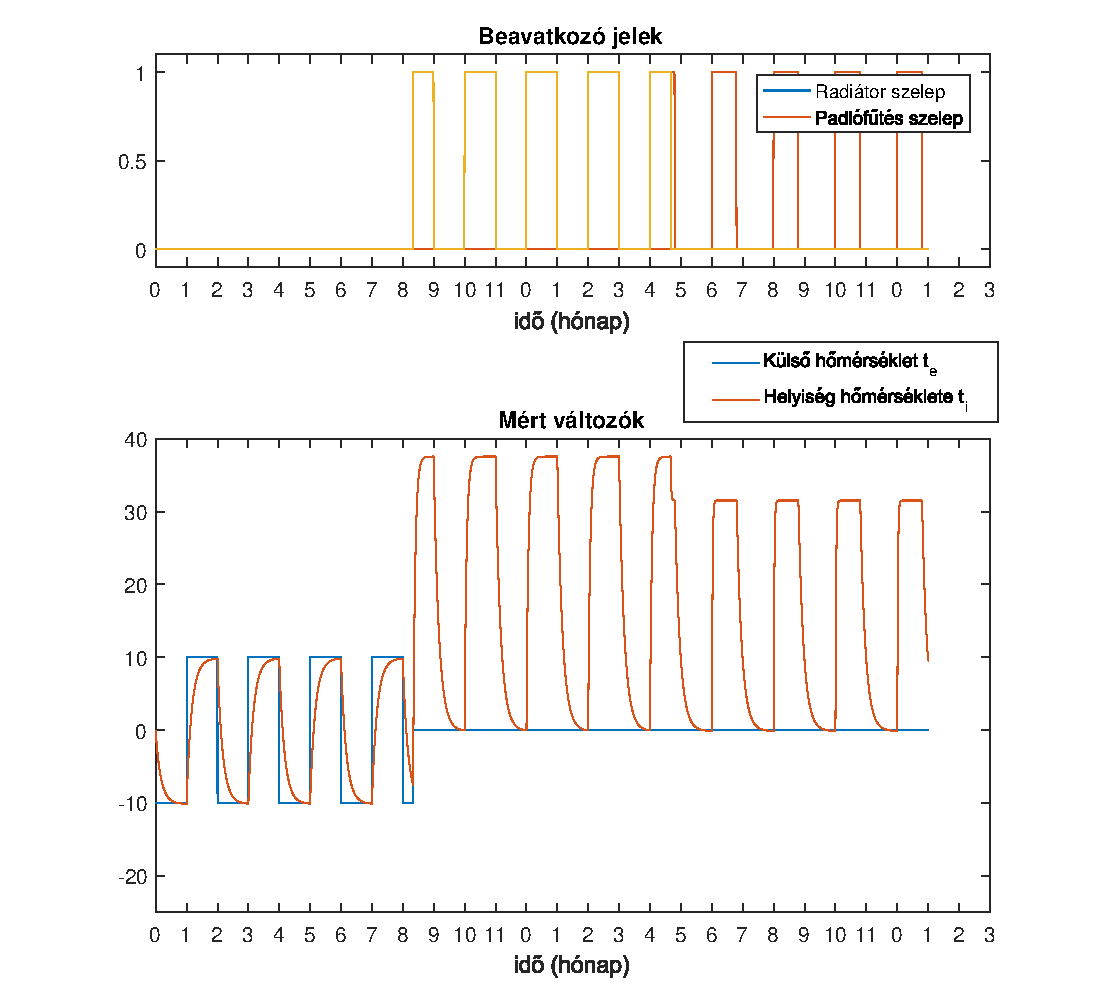
\includegraphics[trim=0 0 0 0, clip,width=\textwidth]{figures/ident-valve3}
	\caption{Identifikáció során }
	\label{fig:ident}
\end{figure}

Az identifikáció pontosságának javításához mindhárom bemeneti változó hatását több periódusra rögzítettem, 750 napnyi szimulációval. Ez fél órás mintavételi idő mellett szimulációban kevesebb, mint 1 perc alatt futott le\footnote{7. generációs i5 processzor, 8GB RAM, SSD használatával}. Az identifikációhoz a hőmérsékletet kelvinben rögzítem, mivel \si{\celsius} használata esetén az összefüggések nem lineárisak. (A kelvinben mért hőmérsékletet nevezik termodinamikai hőmérsékletnek.) A fenti esetben a beállási idők kb. 30 naposak az egész rendszert tekintve, ami kb. 10 napos időállandót jelent. Szakirodalom szerint a falszerkezetek időállandója kb. 5 nap, a helyiségre így reálisnak tűnik a közelítés.

Átviteli függvény identifikációjához a fenti nemlinearitásokat okozó gerjesztéseket nem vettem figyelembe. Így az átviteli függvény a rendszer jellegét követte, és a \textit{\ref{fig:valve-step-hot}. ábrán} látható külső hőmérsékletre és teljesen kinyitott szelepekre a végértékek pontosan illeszkednek.


\begin{figure}[H]
	\centering
	% trim={<left> <lower> <right> <upper>}
	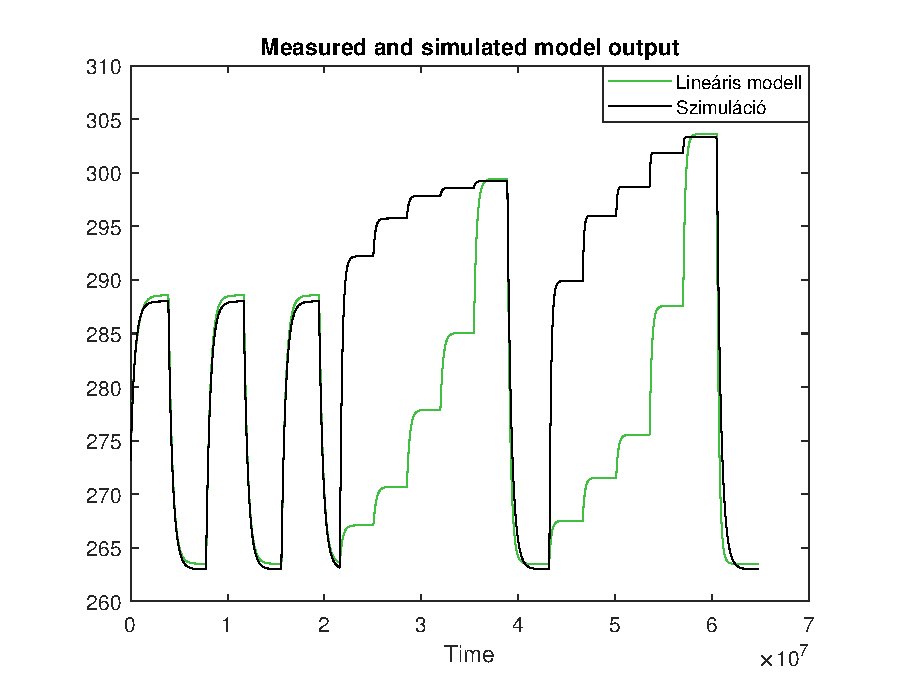
\includegraphics[trim=0 0 0 0, clip,width=0.9\textwidth]{figures/identModelOutputMatch}
	\caption{Identifikált modell pontatlansága}
	\label{fig:ident-model-mismatch}
\end{figure}

%Zérusok hatása röviden. Mit tud. Hánytárolós rendszer. Néhány kép.
%MISO identifikáció. 
%
%
%\section{Hagyományos szabályzás performanciája}
%
%PI, miért nem jó
%Csak SISO-ra működik és itt esetünkben itt több bemenetről van szó mindenképpen. Irodalom: S. Prívara et al. 
%


\pagebreak